% ===========================================================================
% Rate-Register Quantisation Effects in MEMS Gyroscopes
%
% BUILD:   latexmk -pdf main.tex          (or: press Ctrl+Alt+B in VS Code)
% CLEAN:   latexmk -C
%
% NOTHING IN THIS FILE IS THE PAPER. Every section is a stub carrying the
% argument order and the evidence it has to cite. Prose goes in the section
% files under sections/.
% ===========================================================================

% --- TARGET CLASS ----------------------------------------------------------
% Draft (works out of the box):
\documentclass[11pt,a4paper]{article}
%
% IOP Measurement Science and Technology -- download iopart.cls from
%   https://publishingsupport.iopscience.iop.org/questions/latex-template/
% and put it beside this file, then use:
% \documentclass[12pt]{iopart}
%
% IEEE TIM -- IEEEtran.cls ships with TeX Live:
% \documentclass[journal]{IEEEtran}
% ---------------------------------------------------------------------------

\usepackage[T1]{fontenc}
\usepackage{lmodern}
\usepackage[utf8]{inputenc}
\usepackage[british]{babel}
\usepackage{geometry}
\geometry{margin=25mm}

\usepackage{amsmath,amssymb}
\usepackage{graphicx}
\usepackage{booktabs}          % \toprule \midrule \bottomrule -- never \hline
\usepackage{siunitx}
\usepackage[hidelinks]{hyperref}
\usepackage[capitalise,noabbrev]{cleveref}
\usepackage{microtype}\setlength{\parskip}{\baselineskip}



\graphicspath{{../Figures/}}   % figures are NOT copied; they are referenced
                               % where figures.py writes them, so a rerun
                               % updates the PDF

% --- units and symbols -----------------------------------------------------
\sisetup{range-units=single, per-mode=symbol}
\DeclareSIUnit{\dps}{\degree\per\second}
\DeclareSIUnit{\mdps}{\milli\degree\per\second}

\newcommand{\Dlsb}{\Delta}                 % the 16-bit register LSB
\newcommand{\Dref}{\Delta'}                % the 20-bit field lattice, D/8
\newcommand{\rhod}{\rho}                   % sigma / Delta
\newcommand{\phase}{\varphi}               % sub-code phase, EDGE-referenced
\newcommand{\etaq}{\eta}                   % added-power ratio

% --- generated numbers -----------------------------------------------------
% numbers.tex is written by tools/make_numbers.py from summary.csv.
% DO NOT TYPE A NUMBER INTO THE PROSE. Use the macros. If a rerun changes a
% value, the paper changes with it; if you type it, it silently goes stale,
% and this project has already moved a headline residual from 0.393 to 0.018.
% GENERATED BY make_numbers.py -- DO NOT EDIT BY HAND.
% Any edit here is overwritten on the next build and will
% put the paper out of step with the data.
%
% source   : summary.csv
% sha256   : fd8c691e9bcdad68
% commit   : unknown
% generated: 2026-07-29 18:25Z
% records  : 49   axis-measurements: 147

% --- derived from summary.csv ------------------------------------------
\newcommand{\etaRangeHi}{+2.478}
\newcommand{\etaRangeLo}{-0.344}
\newcommand{\etaSpan}{2.82}
\newcommand{\nAxisMeas}{147}
\newcommand{\nOdrPoints}{42}
\newcommand{\nPhasePoints}{48}
\newcommand{\nPhaseSteps}{16}
\newcommand{\nRecords}{49}
\newcommand{\nSpecimens}{2}
\newcommand{\odrResidRMS}{0.0671}
\newcommand{\phaseResidMax}{0.0453}
\newcommand{\phaseResidRMS}{0.0179}
\newcommand{\phaseRho}{0.203}
\newcommand{\phiHi}{0.992}
\newcommand{\phiLo}{0.048}
\newcommand{\residPctOfRange}{0.6}
\newcommand{\rhoDecades}{1.01}
\newcommand{\rhoHi}{1.378}
\newcommand{\rhoLo}{0.136}

% --- from named sources, NOT from the csv ------------------------------
% Update these by hand when the source note changes, and
% keep the citation beside each one.
\newcommand{\arwSpan}{$\times 4.7$}
\newcommand{\biasInstHi}{0.051}
\newcommand{\biasInstLo}{0.006}
\newcommand{\deltaMdps}{61.035}
\newcommand{\histMaxDisc}{0.005}
\newcommand{\refImprovement}{76\%}
\newcommand{\refResidBefore}{0.393}
\newcommand{\stepSizeLadder}{0.499513}
\newcommand{\stepSizeSweep}{0.499151}
\newcommand{\vzeroFourTotal}{450}


% --- draft aids, remove before submission ----------------------------------
\usepackage{xcolor}
\newcommand{\todo}[1]{\textcolor{red}{\textbf{[TODO: #1]}}}
\newcommand{\gap}[1]{\textcolor{orange}{\textbf{[GAP: #1]}}}
\newcommand{\expl}[1]{\textcolor{blue}{\textbf{[EXPLORATORY: #1]}}}

% ===========================================================================

\title{Sub-LSB Alignment Effects in MEMS Gyroscope Rate-Register Quantisation\\}
\author{J. Rhodes}
\date{\today}

\begin{document}
\maketitle

\begin{abstract}
\todo{$\sim$200 words. Order: practice $\rightarrow$ gap $\rightarrow$ what was
measured $\rightarrow$ result $\rightarrow$ consequence. Lead with the transfer
rule, not with quantisation theory: the reader must know what breaks before
they can care why. Must contain ``truncating rate register'', ``$-1/2$ slope'',
``two measured parameters'', ``no free parameters'', and one number ---
suggested \etaRangeLo{} to \etaRangeHi{}, or the \arwSpan{} span in fitted ARW.}
\end{abstract}

\section{Introduction}
\label{sec:intro}

% ---------------------------------------------------------------------------
% ~900 words. Argument order, one paragraph each:
%
%  1. Stochastic IMU calibration fits N, B, K from an Allan or wavelet
%     analysis and transfers them across configuration by a sqrt(ODR) rule.
%  2. That rule is stated as a CONDITION in Kalibr's own documentation --
%     requiring ideal decimation -- not as a validated result.
%  3. The standards construct that WOULD model register quantisation, the
%     IEEE-952 angle-quantisation term Q, describes angle-INCREMENT outputs.
%     Wrong architecture for a rate register.
%  4. So for a rate register the term is unmodelled, lands on the -1/2 family,
%     and is absorbed silently into fitted ARW.
%  5. Contributions, four bullets, in Concept Note v2.3 Z.3's survivability
%     order (strongest first).
%
% WHAT IS NOT CLAIMED -- one sentence each, IN the introduction, not buried:
%   - not a new quantiser theory (Bennett, Sripad-Snyder, Widrow-Kollar)
%   - scale factor / misalignment are a different family (IMU-TK)
%   - the effect vanishes at high rho; this is a low-rho paper
% ---------------------------------------------------------------------------

\gap{Kalibr verbatim quote. Concept Note v2.3 Z.5 names this the paper's
weakest structural point and Critical Analysis v2.1 Z.1 makes it a condition
of publishability. Half a day at a desk. Until it is here, \cref{sec:conseq}
overreaches.}

\todo{Write.}

\section{Background and related work}
\label{sec:background}

% ---------------------------------------------------------------------------
% ~800 words.
%
% Cite Bennett (1948), Sripad & Snyder (1977), Widrow & Kollar (2008)
% OURSELVES, as the foundation. Objections v2.1 Z.2 is explicit: the "this is
% Bennett with a gyroscope attached" objection must be pre-empted by citing
% Bennett first, not conceded later.
%
% Then IEEE-952 Q and why it is the wrong architecture for a rate register.
% Then Table 1.
%
% FRAMING FOR TABLE 1 -- this wording is load-bearing and a referee will
% check it. From GMWM-to-Kalman-Q v1.2 Z.4:
%
%   The surveyed pipelines DO NOT MODEL register quantisation AT ALL. It is
%   absent from the model set, not approximated within it.
%
% Do NOT write "they adopt the Delta^2/12 model and it is invalid". That is
% false. The gap is total, which is a STRONGER result, not a weaker one.
% ---------------------------------------------------------------------------

\begin{table}[t]
\centering
\caption{Stochastic calibration pipelines. \todo{From GMWM-to-Kalman-Q v1.2
\S3, with its Z.4 correction applied.}}
\label{tab:toolchains}
\begin{tabular}{lcccc}
\toprule
Pipeline & $\sqrt{\mathrm{ODR}}$ transfer & Models register
         & Exposes $\rhod$ & Assumes \\
         &                                & quantisation
         & or $\mu$        & PQN \\
\midrule
Kalibr              & stated as a \emph{condition} & no & no & implicitly \\
\texttt{allan\_variance\_ros} & yes & no & no & implicitly \\
\texttt{imu\_utils}          & yes & no & no & implicitly \\
GMWM (\texttt{simts}/\texttt{wv}) & per-config fit & IEEE-952 $-1$ only & no & implicitly \\
MATLAB Sensor Fusion & yes & no & no & implicitly \\
NaveGo              & yes & no & no & implicitly \\
\bottomrule
\end{tabular}
\end{table}

\gap{Every row needs a citable source -- documentation URL with access date,
or a source-file line reference. This table is the paper's empirical
foundation for the claim that the misattribution is universal rather than a
strawman, so it must be checkable line by line.}

\todo{Write.}

\section{Theory}
\label{sec:theory}

% ---------------------------------------------------------------------------
% ~1200 words. ONLY what the results need. Critical Analysis v2.1 Z.2 warns
% that the real risk to this paper is depth, not niche: the instinct to
% include every derivation serves the internal corpus and works against a
% journal submission. Full phase-dependent derivations and the H0-H3 tables
% go to supplementary.
%
% Keep: truncating quantiser; the sawtooth series; eta = 12[2Cov(u,e)+Var(e)];
% Gaussian input collapsing onto g_k = exp(-2 pi^2 k^2 rho^2); eta(rho,phi)
% and its two limits.
%
% STATE THE PHASE CONVENTION TWICE. Edge-referenced here, and
% phi_TN14 = phi - 1/2 when comparing with the pre-campaign tables.
% ---------------------------------------------------------------------------

\subsection{The quantiser}
\todo{Write. $Q(x)=\Dlsb\lfloor x/\Dlsb\rfloor$ -- truncation, established by
measurement in \cref{sec:arch}, not assumed.}

\subsection{Added power}
\todo{Write.}
\begin{equation}
  \etaq(\rhod,\phase) = 12\left[\,2\,\mathrm{Cov}(u,e) + \mathrm{Var}(e)\,\right]
  \label{eq:eta}
\end{equation}

\subsection{Symbol conventions}
% NON-NEGOTIABLE. Vaccaro & Zaki (2012) use R for the ARW density and Q for
% RRW, which collides with IEEE-952's Q AND with the Kalman Q/R. A reader
% from either community will misread the paper without this table.
\begin{table}[h]
\centering
\caption{Symbols, with the collisions named explicitly.}
\label{tab:symbols}
\begin{tabular}{llll}
\toprule
Symbol & Meaning & Units & Note \\
\midrule
$\Dlsb$   & 16-bit register LSB & \si{\mdps} & \num{61.035} at \SI{\pm2000}{\dps} \\
$\Dref$   & 20-bit field lattice & $\Dlsb$ & $\Dlsb/8$; see \cref{sec:refquant} \\
$\rhod$   & $\sigma/\Dlsb$, dither ratio & --- & the independent variable \\
$\phase$  & sub-code bias phase & $\Dlsb$ & \textbf{edge}-referenced \\
$\etaq$   & added power $/(\Dlsb^2/12)$ & --- & $+1$ is the classical limit \\
\bottomrule
\end{tabular}
\end{table}

\begin{figure}[t]\centering
  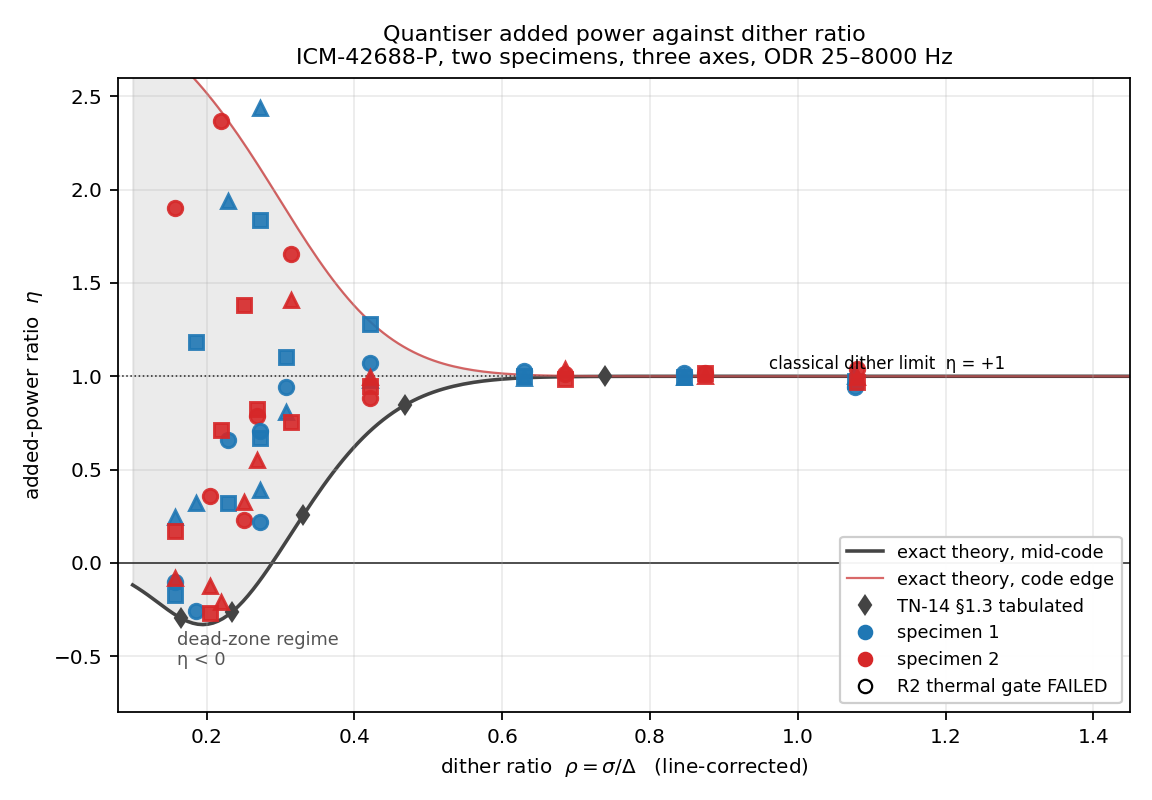
\includegraphics[width=\linewidth]{fig1_eta_vs_rho.png}
  \caption{\todo{$\etaq$ against $\rhod$, with the band spanning all phases.}}
  \label{fig:etarho}
\end{figure}

\section{Instrumentation and Statistical Methods}
\label{sec:method}
% ~1000 words.



\subsection{Instrument}
The experiment used a custom PCB, consisting of two ICM-42688-P MEMS gyroscopes. The standard 16-bit channel of the ICM-42688-P and the extended 20-bit channel (read from the FIFO buffer) were both read simultaneously over the same physical samples. The use of the 20-bit channel  forces the full-scale range (FSR) to $\pm$\SI{2000}{\degree\per\second} due to a limitation in the device \todo{reference datasheet?}. The relationship between the two is determined in \todo{S5.1 likely}. The two ICM-42688-P devices are referenced as specimen 1 and specimen 2 within the manuscript.

A STM32F723ZET6 microcontroller unit (MCU) was used to collect the sensors readings and log the data to an SD card.  Throughout the experiment, all clock speeds (such as the chosen 32MHz SYSCLK for the MCU, and 8MHz SPI clocks) were kept intentionally constant and low as an experimental control. This was done to avoid the increased electrical noise that occurs with higher clock speeds that could couple into the sensors and act as dither, abolishing the effect under study. Power was supplied through a power-only USB cable with data lines disconnected instead of a battery during all datalogging, as it was found in preliminary testing that the larger connected ground plane reduced a persistent spectral spur. The spur was measured at \SI{119}{\hertz}, with an amplitude of $1.28\Delta$ on battery against $0.42\Delta$ on USB, unknown exact source \todo{further detail?}, which would reduce the gaussianity that the model assumes.

Throughout the experiment, the devices where measured at ODRs of \SIlist{25;50;100;200;500;1000;8000}{\hertz}, and with the AAF filter set to bandwidths of \todo{confirm AAF filter settings range, DS-000347}. The record durations of \todo{confirm record durations}, where derived from \todo{calculatiosn for duration if relevant, cant just say vibes}.



\subsection{Reference channel quantisation}
\label{sec:refquant}
% A genuine methods contribution, and the most transferable thing in the
% paper: anyone using a higher-resolution channel as ground truth for a
% lower-resolution one has this problem and will not have corrected for it.
%
% MUST COME BEFORE THE ESTIMATORS. See the note at the head of this file.
%
% THE THREE PLACES IT ENTERS. This is the structure of the subsection, and
% getting all three named is the whole point -- as of 30 July the campaign had
% applied two of them and left the third, which is what TN-24 is about.
%
%   1. phase     phi read from x is low by Delta'/2 = 1/16 Delta
%   2. width     Var(x) carries Delta'^2/12 of the reference's own noise
%   3. eta       eta's numerator is Var(Q) - Var(v), NOT Var(Q) - Var(x), so
%                it needs +Delta'^2/12 as well -- a constant +1/64 of eta
%
% (3) was missed until 30 July. It left a constant -0.0153 +/- 0.0012 offset
% in every eta in the campaign against a predicted -1/64 = -0.015625, and
% correcting it cut the sweep residual by 39%. Present all three together as
% one correction applied in three places, not as two corrections and a later
% patch: they are the same Delta'^2/12 and the same 1898 paper.
%
% STATE THE FACTOR OF TWO EXPLICITLY OR THE READER WILL THINK YOU ARE WRONG.
% Eq (1) gives x = gyro_20 / 16, from which the field's LSB looks like
% Delta/16 = 0.0625 Delta -- and a reader who does that arithmetic will
% conclude the correction is twice too big. It is not: the 20-bit FIFO format
% carries only 19 significant bits of gyroscope data, so the gyro LSB is
% always zero and the effective lattice is TWO counts,
%     Delta' = 2/16 Delta = Delta/8,
% giving a half-lattice phase offset of Delta'/2 = 1/16 Delta = 0.0625, which
% is what was measured (+0.0623). One sentence naming the 19 significant bits
% closes the gap. Cite TDK for the 19-bit figure -- the product page states
% "19-bits of gyroscope data and 18-bits of accelerometer data"; find it in
% DS-000347 Rev 1.6 and cite the section, not the web page.
%
% WHY PQN IS EXACT FOR THE REFERENCE AND FAILS FOR THE REGISTER -- the one
% sentence that stops this looking like special pleading. The reference
% lattice is 8x finer, so rho' = 8 rho = 1.6-2.0 on these records and the
% Gaussian collapse factor exp(-2 pi^2 rho'^2) is of order 1e-22. The same
% theory that predicts a 250% departure for the register predicts none at all
% for the reference. That is a consistency check, not an excuse.
%
% The cascade is transparent: because Delta' divides Delta exactly,
%     floor( floor(x/Delta') Delta' / Delta ) = floor(x/Delta)
% identically, so Q is unchanged and only Var[x] needs correcting.
\expl{Places 1 and 2 were found by fitting a free offset to a residual, not
predicted in advance; place 3 was found in the residual left by the first two.
The out-of-sample evidence is what makes all three defensible: derived from
the \SI{50}{\hertz} phase sweep on one specimen, applied unchanged to the
independent ODR axis and to a second specimen, \refImprovement{} residual
improvement on data they were not derived from. The magnitude of place 3 is
not fitted at all --- it is $(\Dref/\Dlsb)^2 = 1/64$ exactly, and six
independent groups agree with it to within $1.1\sigma$. Say all of this
plainly rather than presenting any of it as a prediction.}

\begin{figure}[htbp]\centering
  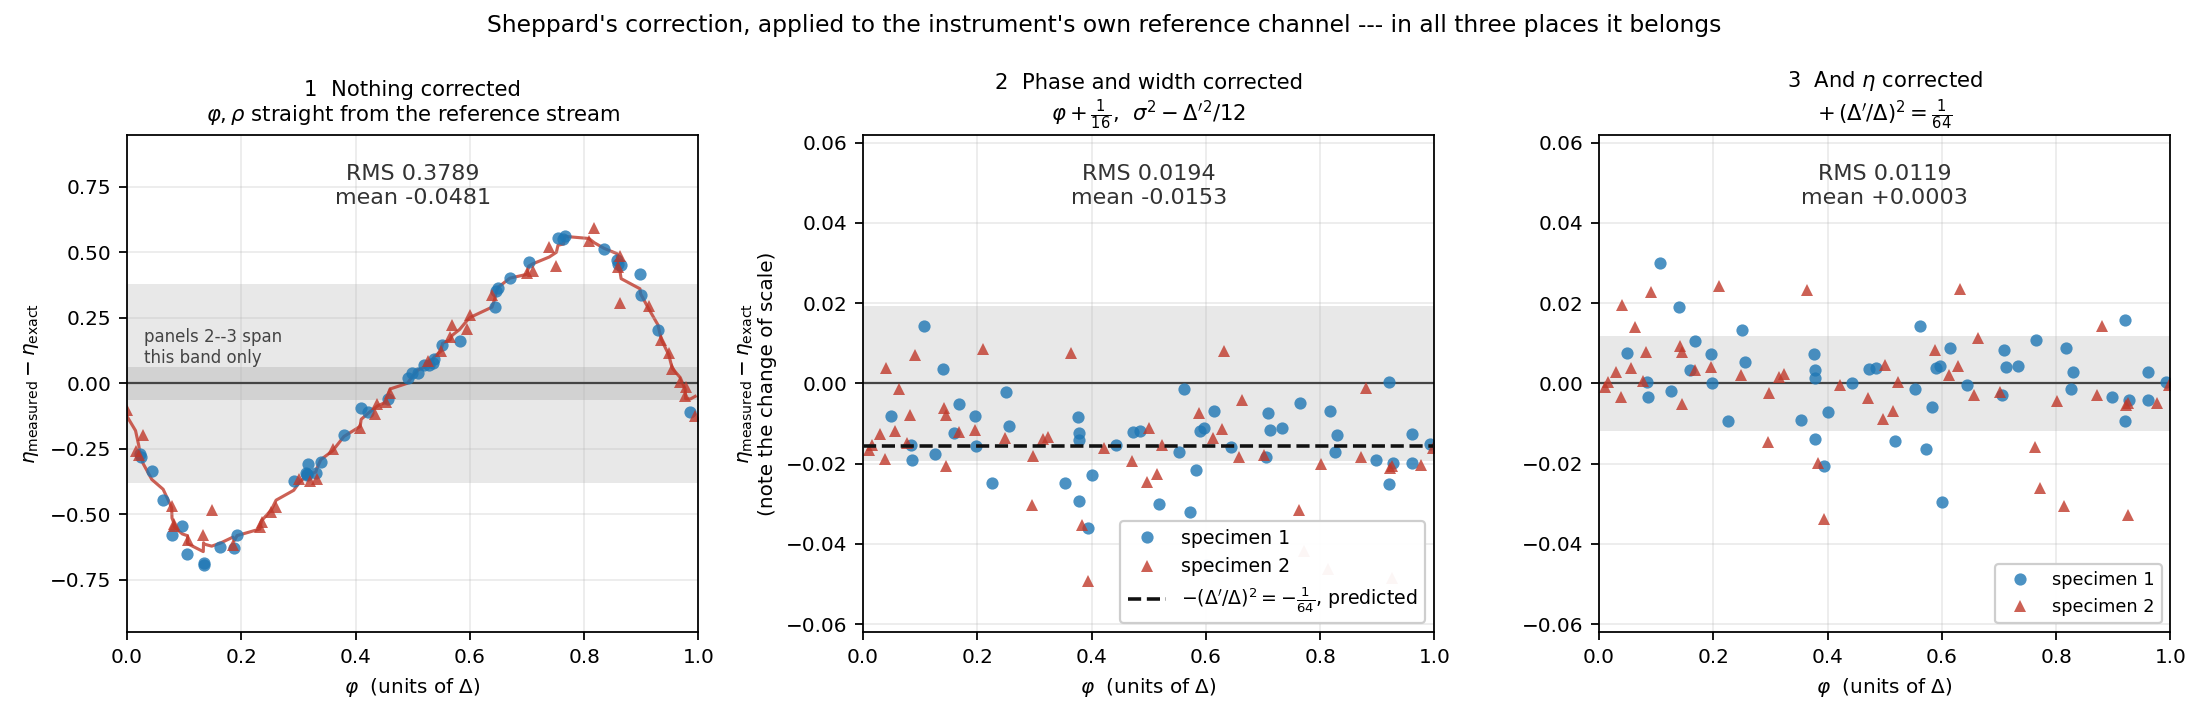
\includegraphics[width=\linewidth]{fig8_reference_truncation.png}
  \caption{\todo{Write. The figure is three panels: nothing corrected,
  $\phase$ and $\rhod$ corrected, and all three places corrected. Both
  specimens are marked separately and lie on top of each other in panel~1,
  which is the point --- the systematic is not specimen-specific. Panel~2
  carries the predicted $-1/64$ line, and panels 2--3 are on a zoomed axis
  (say so in the caption, the reader must not compare spreads across the
  break). RMS $0.379 \to 0.019 \to 0.012$; mean $-0.048 \to -0.015 \to
  +0.000$. No free parameters anywhere.}}
  \label{fig:reftrunc}
\end{figure}

% A SECOND FIGURE BELONGS IN THIS SUBSECTION, or in the results section --
% decide, but do not lose it. The software dither sweep (TN-24 s11) validates
% eta_exact over rho = 0.31 to 3.24 using NONE of the corrections above,
% because there the input to the simulated quantiser genuinely is continuous.
% That makes it the answer to "you corrected the reference until the theory
% fitted": the agreement survives with the correction machinery switched off.
% It also holds rho fixed while ODR changes by 20x, which is the only clean
% answer available to "your rho axis is really an ODR axis".



\subsection{Phase manipulation}
\label{sec:phasectl}
% Procedure, so it belongs before the estimators rather than after them.
%
% OFFSET_USER steps 0.4995 Delta -- so close to half an LSB that a naive
% ladder reaches two phases. The MISS from one half is what makes it sweep.
% A coarse trim register used as a fine phase control.
%
% THE COMMANDED PHASE IS NOT THE MEASURED PHASE, and this is the sentence that
% protects the whole design. The register's job is to MOVE phi, not to place
% it: eta is always evaluated at the phi measured from that record, never at a
% phi computed from the step count. So the 15% uncertainty on the step size
% cannot propagate into the physics. Say it explicitly -- a referee who thinks
% phi was commanded will ask what happens when the command is wrong.
%
% ORDER IN TIME WAS BIT-REVERSED IN k, so corr(phi, time) ~ 0 and any thermal
% drift over a night is orthogonal to the phase axis instead of confounded
% with it. Worth one sentence: it converts a bias into scatter, and the
% ODR-1000 vernier of 30 July shows it working (fit scatter rose, fitted slope
% did not move).
%
% THE STEP SIZE IS ODR-DEPENDENT. [measured] 30 July:
%     ODR 50    0.499157 +/- 0.000013 (vernier)   0.499189 +/- 0.000049 (mu)
%     ODR 1000  0.499503 +/- 0.000020 (vernier)   0.499513 +/- 0.000073 (mu)
% The two estimators agree at each ODR; the two ODRs differ by 14.5 sigma.
% Consequence for THIS section: a k-ladder designed at one ODR does not sweep
% the same phases at another, so the ladder is ODR-specific. Consequence for
% the physics: none, because phi is measured per record. Make both points, in
% that order, and keep the mechanism speculation in the discussion.
%
% COVERAGE COMES FROM THE THREE AXES, NOT FROM k. On specimen 2 the vernier
% period is 1/eps = 2305 steps, longer than the 2047-step register ceiling, so
% one sweep in even k reaches only 0.83 of a period. The axes have different
% intrinsic phases (0.521, 0.340, 0.525) and fill each other's gaps: 3 x 16
% spans phi = 0.011 to 0.998 with a largest gap of 0.056. The edge region,
% where eta peaks at 3 - 12 rho^2, is therefore reached ONLY through the axis
% offsets -- so no axis may be dropped in analysis, and that is a methods
% statement, not a convenience.
\todo{Write. Figure to supplementary: fig9\_vernier.png}



\subsection{Estimators}
\label{sec:estimator}

Two streams were captured for every record. The 20-bit stream served as the reference measurement,
\begin{equation}
  x = \frac{\mathrm{gyro}_{20}}{16},
  \qquad Q = \mathrm{gyro}_{16},
  \label{eq:streams}
\end{equation}

where both $x$ and $Q$ are expressed in units of the register LSB, $\Delta$. By construction, $Q \in \mathbb{Z}$, whereas $x$ is a higher-resolution quantisation of the same underlying continuous rate $v$. As established in \cref{sec:refquant}, the reference lattice is eight times finer than the register lattice ($\Dlsb/\Dref = 8$), though $x$ remains quantised. Let $\mu$ and $\sigma$ denote the mean and standard deviation of $x$. The register is characterised by the following derived quantities:

\begin{equation}
  \rhod = \sqrt{\sigma^{2} - \Dref^{2}/12}, \qquad
  \phase = \left(\mu + \tfrac{1}{2}\Dref\right) \bmod 1, \qquad
  \etaq = \frac{\operatorname{Var}(Q) - \operatorname{Var}(x) + \Dref^{2}/12}
               {\Dlsb^{2}/12},
  \label{eq:quantities}
\end{equation}

Here $\rhod$ denotes the dither ratio, $\phase$ the position of the mean within a code cell, referenced to a code edge, and $\etaq$ is the quantisation noise power introduced by the register, normalised to the PQN model, $\Dlsb^{2}/12$ \todo{reference sheppard -> modern rederivation}.d

All three quantities incorporate the reference-lattice correction derived in \cref{sec:refquant}. The reference quantisation variance, $\Dref^{2}/12$, appears as a subtraction to the variance in the definition of $\rhod$, as the half-cell offset used to reference $\phase$ to a code edge, and as a subtraction from $\operatorname{Var}(x)$ when evaluating $\etaq$. These three corrections are not independent but different manifestations of treating the reference channel $x$ as a quantiser with lattice spacing $\Dref$.

Thus a value of $\etaq = 1$ indicates agreement with the PQN model, whereas a value of $\etaq < 0$ means that the register suppresses variance relative to the unquantised continuous rate $v$. Both $x$ and $Q$ were linearly detrended prior to variance estimation, ensuring that a slow thermal drift does not contribute to their estimated variances.



\subsection{Choice of estimator, and circularity}
\label{sec:circularity}

Throughout the analysis, $\sigma$ was estimated solely from the 20-bit reference stream. Estimating $\sigma$ from the 16-bit code histogram would require fitting a likelihood derived from the memoryless, undithered, uniform quantisation model that is subsiquently tested. This would make the analysis circular. The 16-bit code histogram is reserved as an additional, independent test statistic \cref{sec:histograms}, and is never used to estimate $\sigma$.

% ---------------------------------------------------------------------------
% ONE MORE PARAGRAPH HERE -- precision, and be honest that it is not the
% reason. This is the old PARAGRAPH 3; paragraphs 1 and 2 are the prose above,
% which is now about the right length. Do not let this grow.
%
% The precision gain from using the 20-bit stream is modest: SE(rho) improves
% by 4.9x at ODR 25, 1.7x at 50, 1.3x at 100 and 200, 1.1x at 1000 (TN-14
% s1.2). Largest exactly where the 16-bit histogram collapses toward a single
% code, which is suggestive but not the argument.
%
% Say plainly: the decisive reason is anti-circularity, not precision. A
% referee who thinks you chose the estimator for its variance will not see the
% defence.
%
% Then SE(eta), from the fourth central moment computed by quadrature over the
% quantiser cells rather than assumed Gaussian:
%
%   SE(eta) = (12/Delta^2) sqrt( (mu_4(y) - Var(y)^2) / N * C )
%
% with C a sample-correlation inflation for the ODR-tracking filter.
% GIVE C A PROVENANCE -- an unexplained inflation factor is the first thing a
% referee circles. It is now measurable rather than assumed, from the
% successive-difference ratio: (sigma_diff/sigma)^2 = 1 - r_1, so
% C = (1+r_1)/(1-r_1) for an AR(1) approximation. Measured 30 July:
%     ODR 50, default AAF      sigma_diff/sigma 0.94-0.99  r_1 0.02-0.12  C 1.0-1.3
%     ODR 1000, AAF at floor   sigma_diff/sigma 0.40-0.57  r_1 0.68-0.84  C 5-12
% So C = 1.3 is defensible for the sweep records -- it is the conservative end
% of what was measured -- and badly wrong for the narrow-filter records, where
% SE(eta) is inflated 2.3x to 3.4x. Quote the measured ratio per group rather
% than one global constant, and give the AR(1) formula so C stops being a
% number pulled from nowhere.
%
% AND THE NUMBER THAT MAKES THIS SECTION WORTH READING: an independent
% repeatability estimate now exists. Two sweep points repeated five hours
% later gave sigma_eta = 0.0065 per record (n = 6 pairs, so +/- ~32%), against
% a post-correction sweep residual of 0.0119 RMS over 96 measurements. State
% both. The honest reading is that the theory is good to roughly twice the
% repeatability, not that it is exact -- see TN-24 s5.
%
% REPORTING DISCIPLINE, and it belongs here rather than in the results:
% the headline residual is 0.0119 over ALL 96 measurements. One axis of one
% specimen (slot-2 Y) contributes disproportionately, and without it the
% figure is 0.0091 with every covariate correlation falling below
% significance (TN-24 s9). Report it in that order -- headline, then the
% concentration, then the sensitivity analysis. Quoting 0.0091 as the result
% would be outcome-dependent exclusion, which is the exact thing R2 and R4
% exist to prevent, and a referee who spots it will not believe anything
% else in the section.
%
% The likely cause is worth one clause: slot-2 Y has the highest tail ratio
% sigma/sigma_robust (1.18 against 1.06-1.15), and eta_exact assumes a
% Gaussian input, so a residual tracking departure from Gaussianity is the
% expected failure mode rather than an anomaly.
% ---------------------------------------------------------------------------



\subsection{Record selection}
\label{sec:selection}
% This was PARAGRAPH 4 of a comment block stranded under the circularity
% subsection. It belongs here, last, and it must say WHEN the rules were
% fixed.
%
%   - records excluded only by R2 (thermal), R4 (coherent lines) or a CRC
%     failure; all three specified before the campaign (TN-14 s6, 13 July)
%   - how many records each criterion actually removed. As of 30 July: of the
%     45 records on the third night, zero failed CRC, zero overflowed, zero
%     filled the ring buffer, and every gated record passed R2. Say that
%     plainly -- a selection subsection that excludes nothing is the strongest
%     version of this subsection there is.
%   - R2 is evaluated on the blocked linear drift of the die temperature, NOT
%     the sample range. The range is an extreme-value statistic: at 6e4
%     samples it returns ~8.5 sigma_T and therefore measures the thermometer,
%     not the temperature. Measured on one record: range 823 mK, per-sample
%     sensor noise 84 mK, actual drift 103 mK.
%     ** THIS IS A DEVIATION FROM THE PRE-REGISTERED RULE AND MUST BE FLAGGED
%        AS ONE ** -- it was changed after seeing records fail. The defence is
%        that the statistic was wrong on its own terms, independently of the
%        outcome; make that argument rather than hoping nobody asks.
%   - software versions, and "the analysis was run once". Note honestly that
%     the analysis was RE-run on 30 July when TN-24 corrected eta, and that
%     the correction was applied to every record including those already
%     published in the technical notes, not only to the new ones.
%
% ---------------------------------------------------------------------------
% FORMATTING, applies to the whole section
%   \SI{}{} for every quantity with a unit; \num{} for bare numbers.
%   Number an equation only if something refers to it; \eqref{} to refer.
%   Symbols defined in Table 2 need no redefinition -- point at the table.
% ===========================================================================
\todo{Write, one paragraph, following the brief above.}

\section{Results}
\label{sec:results}

% ~1400 words. ORDER MATTERS: architecture first, because everything
% downstream is conditional on which quantiser this is.
%
% Split the section explicitly into CONFIRMATORY and EXPLORATORY. See
% PREREGISTRATION.md. A reader must be able to tell which is which without
% reconstructing the project's history.

\subsection{Architecture identification}
\label{sec:arch}
% CONFIRMATORY. V0.4 was scored against five pre-specified outcomes
% {rounding, truncation, RPDF, TPDF, neither}.
%
% gyro16 == gyro20 >> 4 exactly. \vzeroFourTotal{} of \vzeroFourTotal{}
% discriminating samples, three ODR spanning 40x, zero ambiguous.
% This is bit-exact and needs no statistics at all -- which is why rule R6's
% likelihood machinery is not invoked (see PREREGISTRATION.md, deviation 4).
\todo{Write.}

\subsection{Added power against dither ratio}
% \nOdrPoints{} axis-measurements, two specimens, rho over \rhoDecades{}
% decades. Residual RMS \odrResidRMS{} against exact theory.
\todo{Write. \cref{fig:etarho}.}

\subsection{Added power against phase: the causal manipulation}
\label{sec:phasesweep}
% THE result. One specimen, one ODR, one configuration; the only thing that
% changes between records is a number written to a trim register.
% \nPhasePoints{} measurements, eta from \etaRangeLo{} to \etaRangeHi{},
% residual RMS \phaseResidRMS{} with ZERO free parameters.
%
% This is what answers Objection #14 part 2 (Objections v2.1 Z.2): phi is
% MANIPULATED, not merely observed.
\todo{Write.}

\begin{figure}[t]\centering
  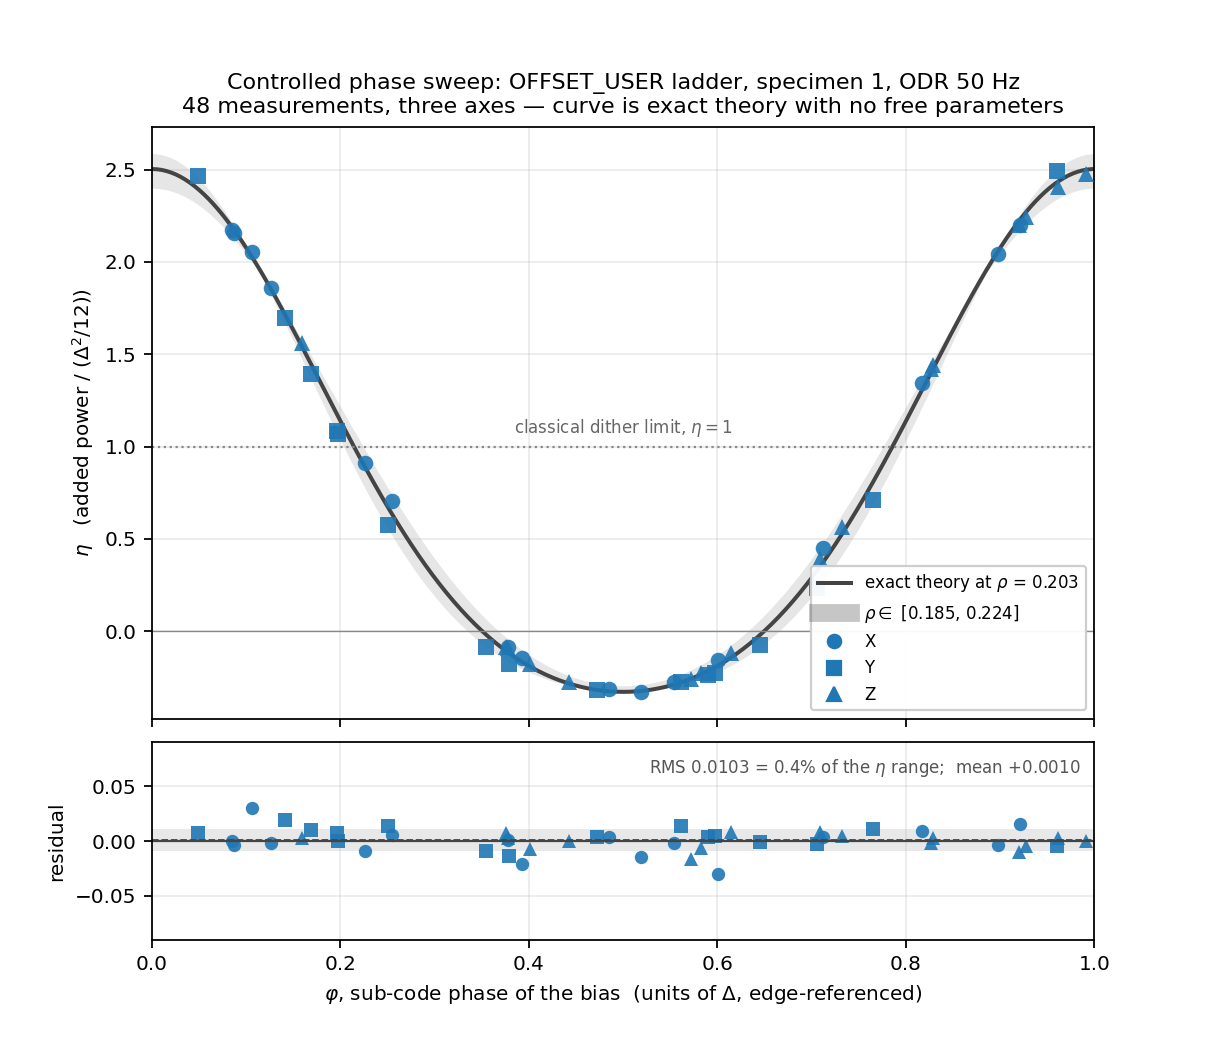
\includegraphics[width=\linewidth]{fig7_phase_sweep.png}
  \caption{\todo{Controlled phase sweep. Curve is exact theory; nothing
  fitted.}}
  \label{fig:phasesweep}
\end{figure}

\subsection{An independent channel}
% Code occupancy, max discrepancy \histMaxDisc{}, nothing fitted. A
% DISTRIBUTIONAL statistic sharing no algebra with eta.
\todo{Write. Figure to supplementary: fig15\_code\_histograms.png}

\subsection{The Allan domain}
% The absence of a -1 slope, with both reference lines anchored ON the data
% so the only thing being compared is the slope.
\todo{Write.}

\begin{figure}[t]\centering
  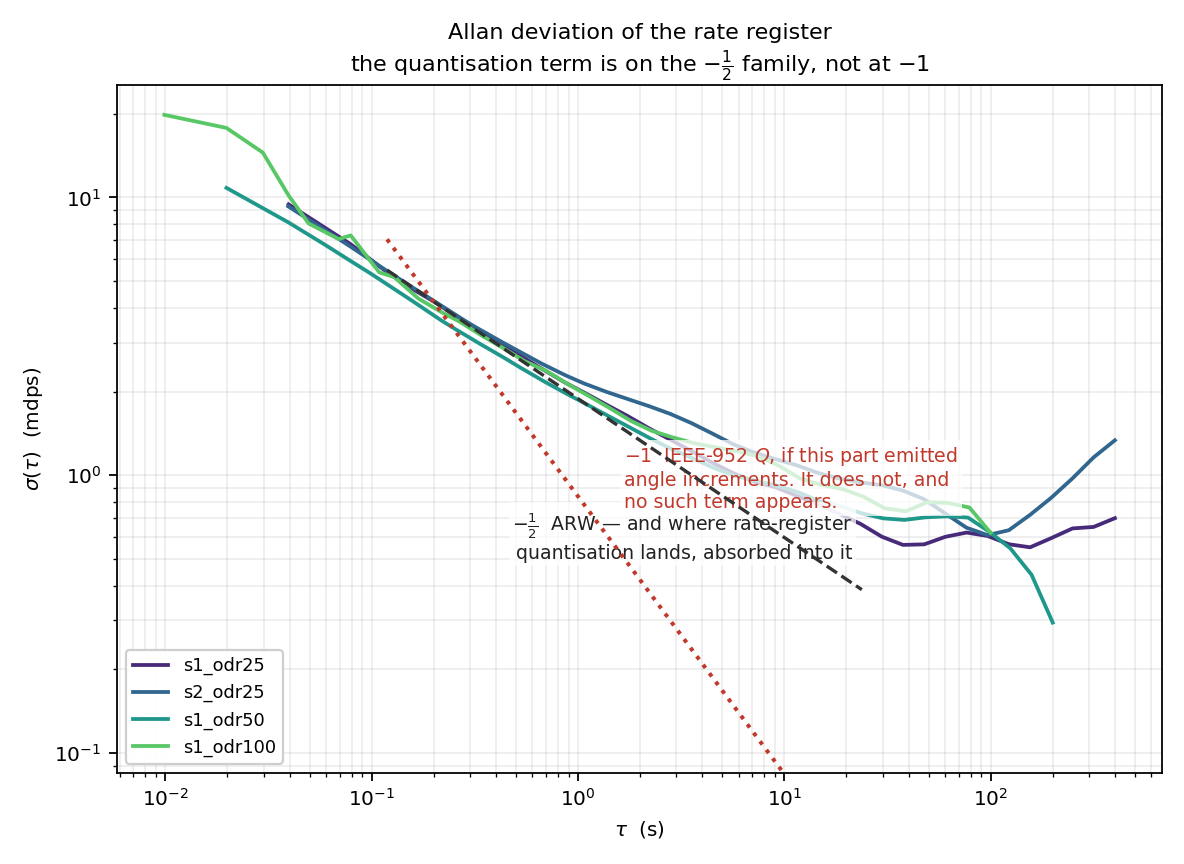
\includegraphics[width=\linewidth]{fig10_allan_family.png}
  \caption{\todo{The quantisation term is on the $-1/2$ family. No
  IEEE-952 $Q$ term appears.}}
  \label{fig:allan}
\end{figure}

\section{Consequences}
\label{sec:conseq}

% ~1000 words. GATED on the relevance evidence -- without it this section
% overreaches and Critical Analysis v2.1 Z.1 says so.

\subsection{At fixed configuration}
% \arwSpan{} in fitted ARW across the phase, same sensor, same settings.
\todo{Write.}

\begin{figure}[htbp]\centering
  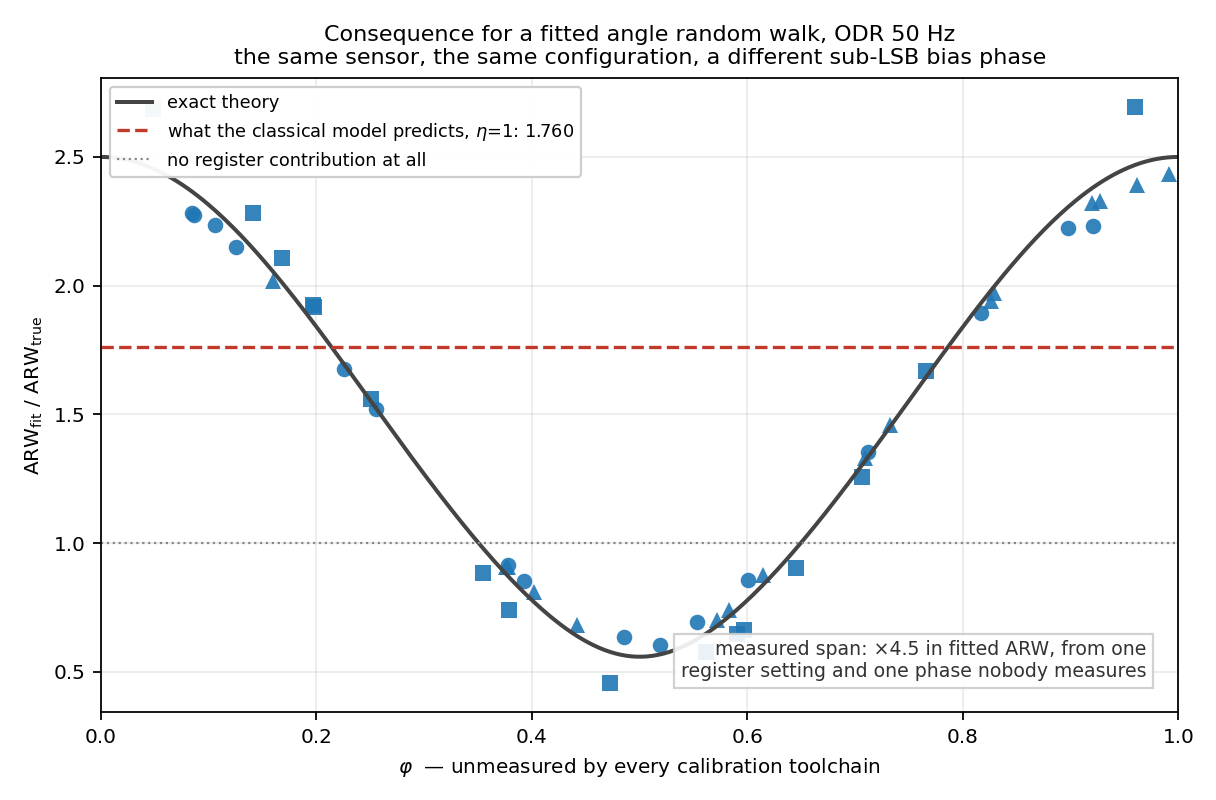
\includegraphics[width=\linewidth]{fig11_arw_consequence.png}
  \caption{\todo{Fitted ARW against the sub-LSB phase no toolchain
  measures.}}
  \label{fig:arw}
\end{figure}

\subsection{Across configuration}
% Three worlds. AS PRACTISED: no quantisation term anywhere. PQN-AWARE: the
% obvious fix, which nobody applies, which is STILL wrong, and which below
% ~69 Hz returns a NEGATIVE noise density. EXACT: right by construction from
% two measured parameters.
%
% The middle world is the point most easily missed and it is
% GMWM-to-Kalman-Q v1.2 Z.2 finding 3.
\todo{Write.}

\begin{figure}[htbp]\centering
  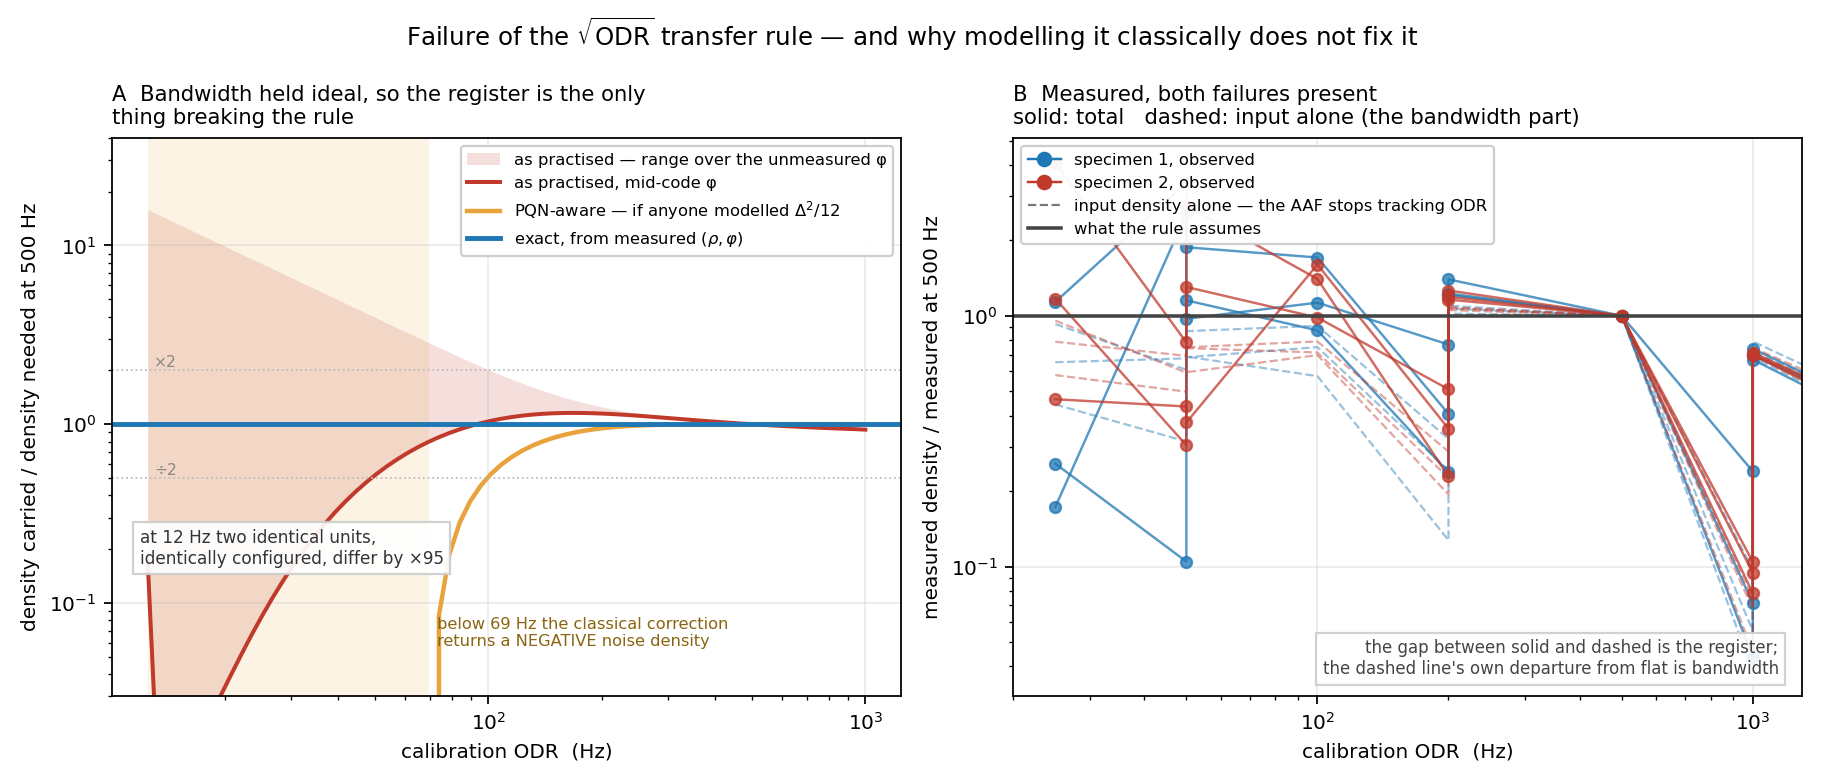
\includegraphics[width=\linewidth]{fig16_transfer_three_worlds.png}
  \caption{\todo{Failure of the $\sqrt{\mathrm{ODR}}$ rule, and why the
  classical correction does not fix it.}}
  \label{fig:transfer}
\end{figure}

\subsection{Locating your own configuration}
% Concept Note v2.3 Z.5 asks for exactly this: a table of effect size against
% ODR at datasheet NBW, so a reader can find their own operating point rather
% than being told about ours.
\todo{Table. Supplementary figure: fig17\_transfer\_surface.png}

\section{Limitations}
\label{sec:limits}

% ~500 words. CONCEDE THESE BEFORE A REFEREE RAISES THEM. Objections v2.1
% Z.1 and Z.2 both say the conceding must happen in the paper, first.
%
%  1. E_mu[G] = 1 EXACTLY. Averaged over units the classical model is
%     unbiased. The error is a per-unit, sign-indefinite gamble -- which is
%     WORSE for someone who owns one sensor than a known bias would be,
%     because a known bias can be corrected. Do not overstate this into a
%     population claim; that version was withdrawn.
%  2. Two specimens, one part number, one FSR, one phase-swept specimen.
%  3. In-record phase stability is limited by bias instability, not by the
%     environment: \biasInstLo{}--\biasInstHi{} Delta.
%  4. The step-size discrepancy of 4.9 sigma, unresolved.
%  5. Bandwidth and register failures are both present in raw data; they are
%     separated in Section 6 but they are not independent in practice.

\todo{Write.}

\section{Conclusion}
\label{sec:conclusion}

% ~250 words. No new claims, no new numbers.
\todo{Write.}


\section*{Data and code availability}
All data and code used to produce the results seen in the paper are publicly available on both Zenodo: (DOI...) and github: (URL...)

\todo{Zenodo DOI and Github URL. All \nRecords{} \texttt{.sdat} records byte-for-byte, the
HDF5 conversions and their converter, the analysis code at its tagged commit,
\texttt{summary.csv}, and a SHA-256 manifest.}

\todo{Notes on deviations}

\bibliographystyle{unsrt}   % iopart-num for MST; IEEEtran for TIM
\bibliography{references}

\end{document}
